\documentclass[10pt,a4paper]{article}
\usepackage[utf8]{inputenc}
\usepackage[T1]{fontenc}
\usepackage{lmodern}
\usepackage[margin=1.5cm, top=1.4cm, bottom=1.4cm]{geometry}
\usepackage{hyperref}
\usepackage{enumitem}
\usepackage{titlesec}
\usepackage{xcolor}
\usepackage{graphicx}

\definecolor{accent}{HTML}{00686E}
\hypersetup{colorlinks=true, urlcolor=accent, linkcolor=accent}
\pagenumbering{arabic}
\setlength{\parindent}{0pt}

\titleformat{\section}{\large\bfseries\color{accent}}{}{0em}{}[\vspace{-0.6em}\rule{\textwidth}{0.8pt}]
\titlespacing{\section}{0pt}{7pt}{4pt}

\newcommand{\role}[4]{%
  \textbf{#1} \hfill \textbf{#2}\\[1pt]%
  \textit{#3} \hfill \textit{#4}\\[2pt]%
}
\setlist[itemize]{leftmargin=1.2em, itemsep=1.5pt, topsep=2pt, parsep=0pt}

\begin{document}

% ================= HEADER =================
\begin{minipage}[c]{0.80\textwidth}
  {\Huge\bfseries Prabhavit Gupta}\\[3pt]
  {\color{accent}\large Automation Solution Architect: Enterprise AI, Agentic Systems \& RAG}\\[6pt]
  {\footnotesize +39 351 610 7807 ~$\vert$~
  \href{mailto:prabhavitg@gmail.com}{prabhavitg@gmail.com} ~$\vert$~
  \href{https://www.linkedin.com/in/prabhavit/}{linkedin.com/in/prabhavit} ~$\vert$~
  \href{https://github.com/prab-gupta}{github.com/prab-gupta} ~$\vert$~
  Venice, Italy (CET Time Zone / EU Permanent Resident)}
\end{minipage}\hfill
\begin{minipage}[c]{0.18\textwidth}
  \raggedleft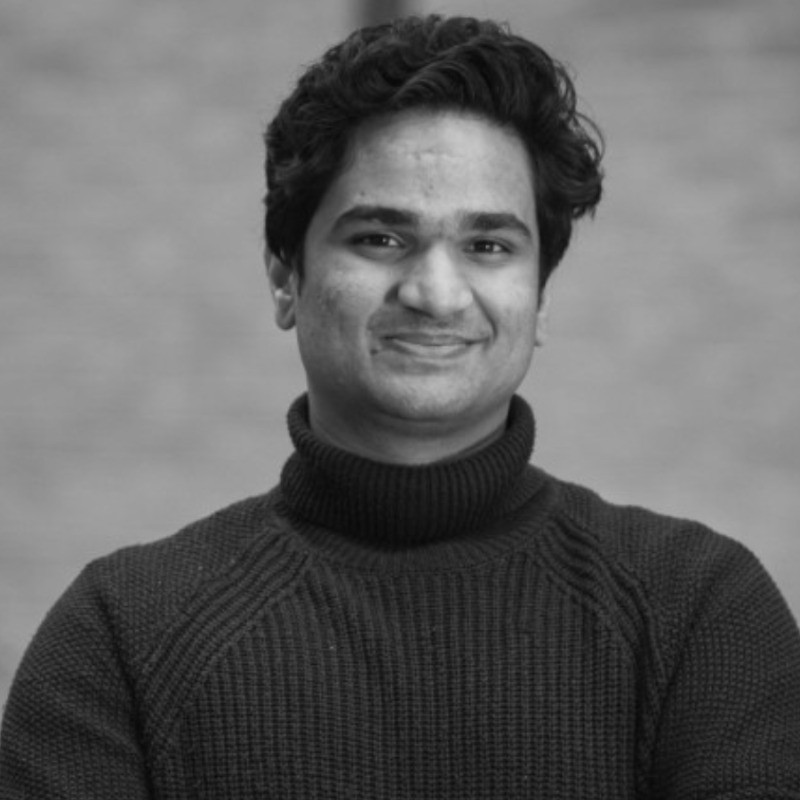
\includegraphics[width=2.0cm]{photo.jpg}
\end{minipage}
\vspace{-2pt}

% ================= SUMMARY =================
\section{Summary}
Automation Solution Architect and Systems Engineer with 3 years of hands-on production experience architecting enterprise automation programmes, greenfield AI pilots, and hybrid agentic workflows. Proven expertise conducting objective feasibility evaluations to balance deterministic automation (workflow engines, n8n, RPA APIs) against generative agentic architectures (tool calling, dynamic context injection, RAG). Skilled in designing human-in-the-loop guardrails, authoring architecture review documentation, and establishing production testing and evaluation standards. Based in Venice, Italy (CET time zone) with registered freelance sole-trader/B2B status and an EU Long-Term Residence Permit (permanent unrestricted EU work authorization, no sponsorship required); available immediately.

% ================= TECHNICAL EXPERTISE =================
\section{Technical Expertise}
\begin{itemize}
  \item \textbf{Automation Solution Architecture:} Greenfield solution design, vendor-neutral tooling evaluation, agentic vs deterministic automation trade-offs, feasibility and cost-benefit modeling, security architecture documentation.
  \item \textbf{Agentic Solutions \& RAG:} Multi-step tool-using agents, LangChain, Model Context Protocol (MCP), prompt and context window strategies, hybrid vector retrieval, human-in-the-loop review gates, safety guardrails.
  \item \textbf{Workflow Automation \& Integration:} n8n, RESTful webhook orchestration, API middleware, asynchronous queues (Redis), document parsing and extraction pipelines, structured JSON schema validation.
  \item \textbf{Software Development \& Cloud:} Python (FastAPI, asyncio, pandas), TypeScript, Node.js, PostgreSQL, GCP (Vertex AI), Docker containerization, GitOps, CI/CD pipeline automation.
  \item \textbf{Quality \& Testing Standards:} Automated evaluation harnesses (golden datasets, precision/recall metrics), end-to-end regression testing with Playwright, contract testing, production observability and error logging.
  \item \textbf{Languages \& Authorization:} English (C1 Professional, fluent), Hindi (Native), Italian (Beginner). EU Long-Term Residence Permit (unrestricted EU work authorization across all EU member states, no sponsorship required).
\end{itemize}

% ================= EXPERIENCE =================
\section{Experience}

\role{\href{https://flowspace.co}{FlowSpace.co}}{Mar 2024 - Aug 2026}{Lead Developer \& AI Systems Architect}{London, UK (remote)}
\begin{itemize}
  \item Architected and delivered greenfield AI automation pipelines and multi-step agentic workflows for an enterprise marketplace serving 4,500+ active users.
  \item Designed a vendor-neutral decision framework balancing deterministic API workflows against generative LLM agents, optimizing running costs, latency, and reliability.
  \item Engineered agentic solutions incorporating MCP tool integrations, dynamic context injection, structured output enforcement, and mandatory human-in-the-loop approval checkpoints.
  \item Authored technical architecture design documentation and security specifications, passing rigorous compliance reviews for enterprise partner integrations.
  \item Implemented automated evaluation harnesses to benchmark agent retrieval accuracy and response grounding against production interaction logs.
  \item Architected high-concurrency backend services using TypeScript, Python (FastAPI), Redis asynchronous queues, and PostgreSQL databases.
\end{itemize}

\role{Urlink}{Apr 2025 - Jul 2025}{Project Manager \& Solutions Developer (Freelance)}{Barcelona, Spain (remote)}
\begin{itemize}
  \item Led technical discovery, solution architecture, and client-facing delivery of automated data processing and integration solutions for European platforms.
  \item Evaluated client operational bottlenecks, architecting webhook-driven automation pipelines connecting third-party SaaS tools to centralized relational databases.
  \item Produced detailed technical specifications, interface diagrams, and integration test plans to guide cross-functional implementation teams.
\end{itemize}

\role{Independent Technical Consultant}{Aug 2023 - Feb 2024}{AI Automation \& Integration Developer}{Venice, Italy}
\begin{itemize}
  \item Consulted European SMBs on automation architecture, implementing custom n8n workflows, webhook integrations, and Vertex AI/LLM pipelines.
  \item Built automated data extraction and validation systems, replacing fragile manual spreadsheet tasks with robust, event-driven pipelines.
  \item Conducted technical workshops with client stakeholders to define automation readiness, error handling policies, and ROI targets.
\end{itemize}

% ================= EDUCATION =================
\section{Education}
\role{Ca' Foscari University of Venice}{2020 - 2024}{BA in Philosophy, International Studies and Economics}{Venice, Italy}
\begin{itemize}
  \item Rigorous training in formal logic, analytical problem solving, systems analysis, and macroeconomic decision models.
\end{itemize}

\end{document}
